\documentclass{article}
\usepackage{pgfplots}
\pgfplotsset{compat=1.9}
\begin{document}

%% 3D Scatter Plot using formula z=sin(2x)+y for x,y \in [0,1]
\begin{figure}
    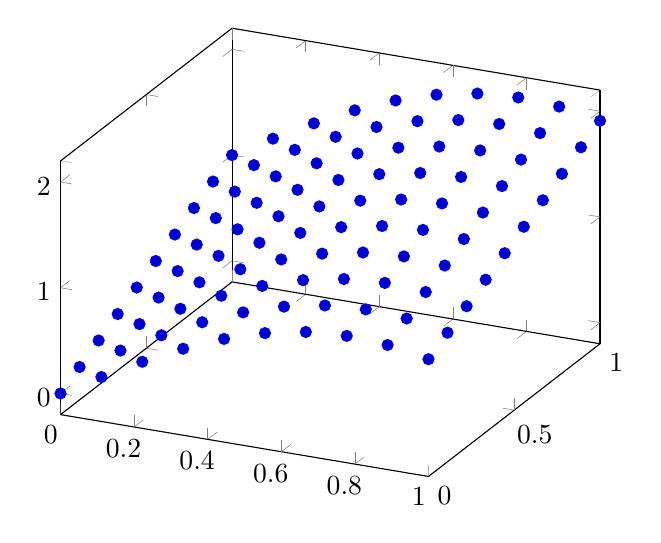
\begin{tikzpicture}
        \begin{axis}
            \addplot3+[only marks,samples=10,domain=0:1]
                {sin(2*deg(x)) + y};
        \end{axis}
    \end{tikzpicture}
\end{figure}

%% Surface Plot using formula z=sin(2x)+y for x,y \in [0,1]
\begin{figure}
    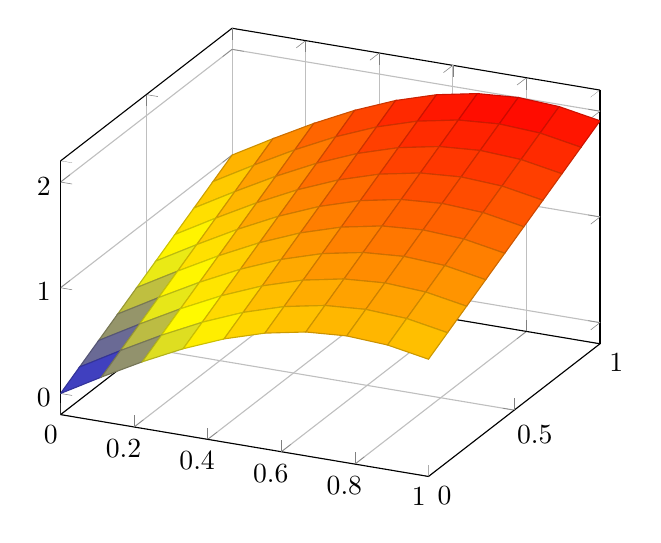
\begin{tikzpicture}
        \begin{axis}[grid=major]%show major axis grid marks
            \addplot3[surf,samples=10,domain=0:1]
                {sin(2*deg(x)) + y};
        \end{axis}
    \end{tikzpicture}
\end{figure}

%% Heat Map
\begin{figure}
    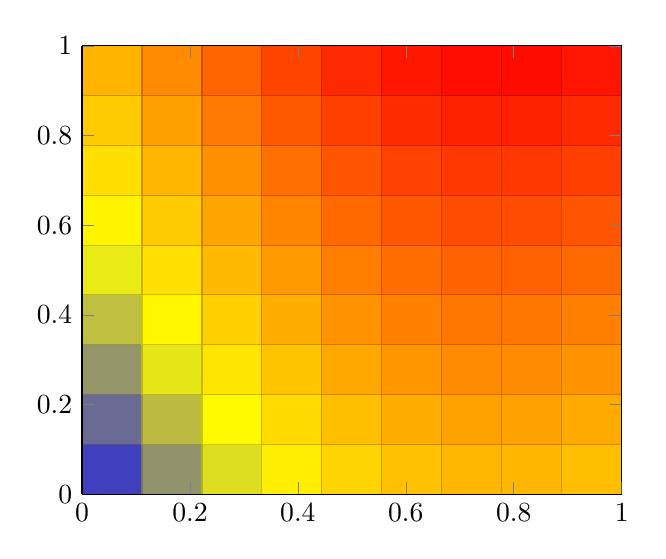
\begin{tikzpicture}
        \begin{axis}[view={0}{90}]%Set view from directly above
            \addplot3[surf,samples=10,domain=0:1]
                {sin(2*deg(x)) + y};
        \end{axis}
    \end{tikzpicture}
\end{figure}

\end{document}
